% !TEX root =  ../Dissertation.tex

\chapter{Methodology}
% The Methodology covers the process for training the Speaker Count CNN and pushing the model to production. First the data collection process is described, followed by the pre-processing required to create the supervised data set of fixed duration voice clips, their spectrograms and the supervision labels. Next, the model architecture is described. Once the architecture was defined and the dataset was prepared, hyperparameter tuning was done with Optuna to find the optimal model hyperparameters, including the number of convolutional layers, skip-connections, optimiser and kernel size. Finally, the method is given for sending the model to a production environment, and how the model was prepared for usage in real-time.

\section{Data Collection}
\label{sec:data_col}
The primary dataset used for model training was LibriCSS \cite{libricss}, a corpus designed to evaluate continuous speech separation systems. It comprises over ten hours of speech from 682 distinct speakers, in clips with varying levels of overlap (Table~\ref{tab:LibriCSS}). Given its overlapping structure and multi-channel recordings, LibriCSS provides a suitable foundation for training a speaker-counting model under pseudo-realistic acoustic conditions.

\begin{table}[H]
  \centering
  \caption{The types of audio present in LibriCSS \cite{libricss}.}
  \label{tab:LibriCSS}
  \begin{tabular}{|l|c|}
    \hline
    \textbf{Audio Type} & \textbf{Meaning} \\
    \hline
    0L (zero-long) & No overlap, inter-utterance gap of $\sim3$ seconds. \\
    \hline
    0S (zero-short) & No overlap, inter-utterance gap of $\sim0.5$ seconds. \\
    \hline
    OV10 (overlap-10) & $\sim10\%$ overlap on utterances. \\
    \hline
    OV20 (overlap-20) & $\sim20\%$ overlap on utterances. \\
    \hline
    OV30 (overlap-30) & $\sim30\%$ overlap on utterances. \\
    \hline
    OV40 (overlap-40) & $\sim40\%$ overlap on utterances. \\
    \hline
  \end{tabular}
\end{table}

\noindent As the majority of LibriCSS samples contain overlapping speech, the dataset provided an insufficient number of zero-speaker `noise' samples. To address this imbalance the Room Impulse Response and Noise (RIR\&N) database \cite{RoomImpulseResponseDatabase} was incorporated into the training set. RIR\&N contains approximately 45 minutes of non-speech audio, including white noise, reverberation, and ambient recordings. In addition, supplementary noise clips were recorded to further expand the zero-speaker class. These recordings were collected under varied conditions to capture a broader range of acoustic characteristics (Table~\ref{tab:authordata}), resulting in approximately 125 minutes of new data. In total the combined dataset amounted to roughly 13 hours of audio for pre-processing (Table~\ref{tab:datacollection}).


\begin{table}[H]
  \centering
  \caption{A description of each manually recorded audio file. Different noise levels and sources were incorporated to give the greatest possible variance in the data.}
  \label{tab:authordata}
  \begin{tabular}{|l|c|l|c|}
    \hline
    \textbf{Audio File} & \textbf{Duration} & \textbf{Description} & \textbf{Average Noise Level}  \\
    \hline
    Downstairs 1 & 00:20:00 & Walking around, indoor ambience & Low \\
    \hline
    Downstairs 2 & 00:05:00 & Doing chores & High \\
    \hline
    Upstairs 1 & 00:02:00 & Working at a desk & Medium \\
    \hline
    Upstairs 2 & 00:07:00 & Doing chores, eating a snack & Medium \\
    \hline
    Upstairs 3 & 00:01:00 & White noise & High \\
    \hline
    Upstairs 4 & 01:30:00 & Left by a window; occasional cars passing \& animal sounds & Low \\
    \hline
  \end{tabular}
\end{table}


\begin{table}[H]
  \centering
  \caption{The amount of audio collected from each source.}
  \label{tab:datacollection}
  \begin{tabular}{|l|c|}
    \hline
    \textbf{Data Source} & \textbf{Duration}  \\
    \hline
    LibriCSS & $\sim$10 hours \\
    \hline
    Room Impulse Response \& Noise (RIR\&N) & $\sim$45 minutes \\
    \hline
    Author added samples & $\sim$2 hours \\
    \hline
    \textbf{Total} & 12:53:13 \\
    \hline
  \end{tabular}
\end{table}

\section{Data Pre-Processing}
\label{sec:data_preproc}
Each recording was downmixed to a single channel (mono) to emulate the conditions of a single-channel recording. While this increased the difficulty of the learning task, it enhanced the model's applicability to real-world scenarios where multi-microphone arrays are typically unavailable. The LibriCSS corpus was originally captured using a seven-channel setup \cite{libricss}, providing rich spatial information that facilitates separation and recognition; such configurations are impractical in real-world applications.\newline

\noindent Following downmixing, the audio was segmented into fixed-length clips of one second and a sample rate of 16,000Hz. The use of a consistent clip duration and sample rate was necessary to standardise input lengths for the neural network, ensuring comparability across samples and maximising learnability. This duration and rate was selected as it provided sufficient temporal context for distinguishing between speakers whilst also maintaining a manageable input size for efficient training and inference.

\begin{figure}[H]
  \centering
  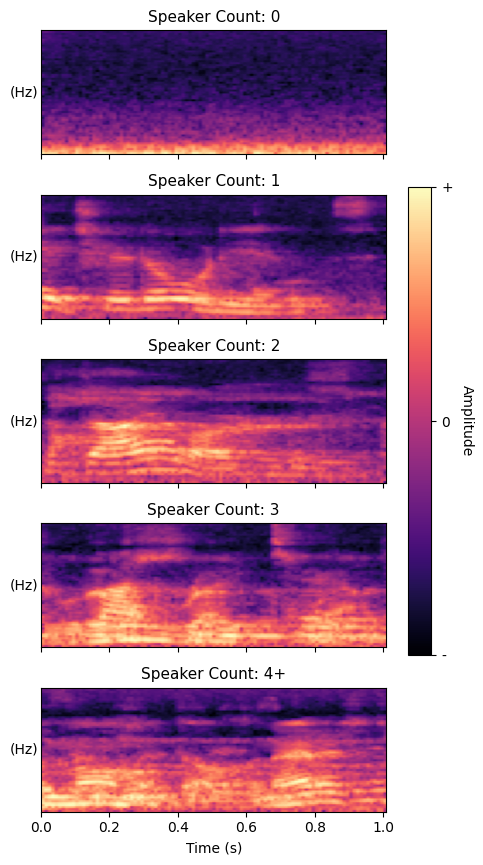
\includegraphics[scale=0.75]{figs/Methodology/SpectrogramExample.png}
  \caption{A series of spectrograms created with the \lstinline!SpectrogramExtractor()! class on speech audio. Speaker count was found by manually cross-referencing the audio's source metadata (Appendix \ref{app:libricss_metadata}). Spectral activity appears to increase with speaker count. With a low number of speakers ($n = 1, 2$) the spectral patterns of each speaker are visible, including higher multiple harmonics, whereas the result becomes increasingly obscure and noisy as speaker count increases. This suggests that learnability diverges as $n$ increases.}
  \label{fig:spec_samples}
\end{figure}

To create the training samples, a custom pre-processing class \lstinline!SpectrogramExtractor()! was implemented. This class transforms an audio clip into its corresponding spectrogram representation, which stores frequency, amplitude and temporal information in a single sample. By converting the signal into the time-frequency domain, the resulting spectrograms are learnable by a neural network with convolutional layers. The \lstinline!SpectrogramExtractor()! class was used on each clip to create 46,393 spectrograms (Figure~\ref{fig:spec_samples}).\newline

\noindent After creating the spectrograms for each sample, the LibriCSS metadata files (Appendix~\ref{app:libricss_metadata}) were scraped to find the speaker count and speaker ID(s) for each spectrogram. The number of speakers was used as the supervision label for each spectrogram in model training. The noise samples were labelled with $\text{Speaker Count} = 0$. The resulting labelled dataset was formatted as a DataFrame (Table~\ref{tab:libricss_labels}).


\begin{table}[H]
  \centering
  \caption{An extract of the resulting dataset from using the LibriCSS metadata (Appendix~\ref{app:libricss_metadata}) to find the number of speakers for each observation.}
  \label{tab:libricss_labels}
  \begin{tabular}{|l|l|c|l|}
    \hline
    \textbf{Spectrogram Directory} & \textbf{Clip Directory} & \textbf{Speaker Count} & \textbf{Speakers} \\
    \hline
    .../OV40\_session9\_clip90.pt & .../OV40\_session9\_clip90.wav & 2 & \texttt{['1995', '2961']} \\
    \hline
    .../OV40\_session9\_clip91.pt & .../OV40\_session9\_clip91.wav & 1 & \texttt{['2961']} \\
    \hline
    .../OV40\_session9\_clip92.pt & .../OV40\_session9\_clip92.wav & 1 & \texttt{['2961']} \\
    \hline
    .../OV40\_session9\_clip93.pt & .../OV40\_session9\_clip93.wav & 1 & \texttt{['2961']} \\
    \hline
    .../OV40\_session9\_clip94.pt & .../OV40\_session9\_clip94.wav & 1 & \texttt{['2961']} \\
    \hline
    .../OV40\_session9\_clip95.pt & .../OV40\_session9\_clip95.wav & 1 & \texttt{['2961']} \\
    \hline
    .../OV40\_session9\_clip96.pt & .../OV40\_session9\_clip96.wav & 1 & \texttt{['2961']} \\
    \hline
    .../OV40\_session9\_clip97.pt & .../OV40\_session9\_clip97.wav & 2 & \texttt{['2961', '7176']} \\
    \hline
    .../OV40\_session9\_clip98.pt & .../OV40\_session9\_clip98.wav & 2 & \texttt{['2961', '7176']} \\
    \hline
    .../OV40\_session9\_clip99.pt & .../OV40\_session9\_clip99.wav & 2 & \texttt{['2961', '7176']} \\
    \hline
  \end{tabular}
\end{table}

\subsubsection{Evaluating the Dataset}
The dataset currently contained only three speaker count classes [0, 1, 2], preventing a model trained on this data from generalising to scenarios involving three or more speakers. Additionally, the dataset exhibited substantial class imbalance (Table~\ref{tab:samples_pre_aug}), which could have biased model training toward the more frequently occurring classes. To resolve this the dataset was augmented.

\begin{table}[H]
  \centering
  \caption{Number of samples per speaker count before augmentation.}
  \label{tab:samples_pre_aug}
  \begin{tabular}{|c|c|}
    \hline
    \textbf{Speaker Count} & \textbf{Samples} \\
    \hline
    0 & 11719 \\
    \hline
    1 & 29309 \\
    \hline
    2 & 5251 \\
    \hline
  \end{tabular}
\end{table}

%----------------------------------------------------------
\subsection{Data Augmentation}
Data augmentation was employed to address the class imbalance present in the dataset, as well as the lack of samples representing higher speaker counts. Two methods were considered to address the imbalance; $a)$ increase samples in underrepresented classes, or $b)$ reduce samples in overrepresented classes. Option $b$ was simpler however valuable information could be lost. Option $a)$ was therefore chosen and alternative data sources were considered to increase class sizes. To create higher speaker audio, synthetic samples were generated by selecting pairs of clips and combining them. The clips were overlayed and normalised to produce realistic multi-speaker recordings. The spectrograms were extracted from the new clips via the usual process with \lstinline!SpectrogramExtractor()!. Finally, the speaker counts for the synthetic samples were created by summing the counts of the original clips, and the observations were added to the dataset.\newline

\noindent Clip selection was pseudo-random; clips were separated into groups by their number of speakers first, and samples were then drawn from two chosen groups to make a pair. This meant that the number of samples for each class could be curated, and class balance was possible (Table~\ref{tab:augmentation_summary}). Additionally, checks were made using speaker ID to ensure that clips of the same speaker weren't overlayed, as combining two clips of the same voice could be interpreted as a single speaker. It was noticed that if a speaker began talking in the first or last milliseconds of a clip the speech wouldn't be audibly significant, so counting the speech would be inappropriate. A minimum utterance length of $0.2$ seconds was set for labelling, so that insignificant speech couldn't distort the speaker count labels. Table~\ref{tab:samples_aug} shows the final class counts after augmentation. \newline

\noindent The final class sizes were curated to reflect both the difficulty of the class to learn and its occurrence in the world. For example, the `0' class, where observations are only silence and noise, was theoretically easier to learn than the higher classes, so less observations were needed. In contrast the `1' speaker class is the most common class in the real-world, so there are more observations for this class than the others. With this in mind, a strategically weighted dataset was created.

\begin{table}[H]
  \centering
  \caption{Summary of data augmentation for multi-speaker classes. The original dataset was split into `0-speaker', `1-speaker' and `2-speaker' samples. These could then be overlayed to create a clip with any number of speakers.}
  \label{tab:augmentation_summary}
  \begin{tabular}{|c|c|c|c|}
    \hline
    \textbf{Base Clips} & \textbf{Overlay Clips} & \textbf{Resulting Speaker Count} & \textbf{Samples Created} \\
    \hline
    1-speaker & 1-speaker & 2 & 17,500 \\
    \hline
    0-speaker & 2-speaker & 2 & 2,500 \\
    \hline
    2-speaker & 1-speaker & 3 & 25,000 \\
    \hline
    2-speaker & 2-speaker & 4+ & 10,000 \\
    \hline
    3-speaker & 1-speaker & 4+ & 7,500 \\
    \hline
    3-speaker & 2-speaker & 4+ & 7,500 \\
    \hline
  \end{tabular}
\end{table}




\begin{table}[H]
  \centering
  \caption{Number of samples per speaker count after augmentation.}
  \label{tab:samples_aug}
  \begin{tabular}{|c|c|}
    \hline
    \textbf{Speaker Count} & \textbf{Samples} \\
    \hline
    0 & 11,719 \\
    \hline
    1 & 29,309 \\
    \hline
    2 & 25,251 \\
    \hline
    3 & 25,000 \\
    \hline
    4+ & 25,000 \\
    \hline
  \end{tabular}
\end{table}

\subsubsection{Changes for the Voice Activity Detection (VAD) task}
\label{sec:vad_labels}
For the VAD task speaker labels needed to be altered (Table~\ref{tab:VAD_data_change}). VAD is a binary classification task so only two classes, `speech' (1) and `no speech' (0) are required.

\begin{table}[H]
\centering
\caption{A comparison of the label structure for the Speaker Counting model and the Voice Activity Detection (VAD) model.}
\label{tab:VAD_data_change}
\begin{tabular}{|c|c|c|}
\hline
\textbf{Number of Speakers} & \textbf{Speaker Count Label} & \textbf{VAD Label} \\
\hline
0 & 0 & 0\\
\hline
1 & 1 & 1\\
\hline
2 & 2 & 1 \\
\hline
3 & 3 & 1 \\
\hline
4 & 4+ & 1 \\
\hline
5 & 4+ & 1 \\
\hline
\end{tabular}
\end{table}


%----------------------------------------------------------
\section{Model Architecture}
Artificial neural networks with convolutional layers were employed to extract feature maps from the spectrogram inputs. Convolutional layers efficiently captured local patterns in both time and frequency, making them well-suited for processing audio representations. Long Short-Term Memory (LSTM) and transformer-based architectures were considered, but were deemed less suitable due to higher computational cost and slower inference; convolutional neural networks (CNNs) achieved efficient feature extraction with substantially lower overhead, making them a suitable choice for real-time inference.

\subsection{Architecture for the Voice Activity Detection (VAD) model}
Voice Activity Detection (VAD) was implemented using a compact CNN, designed to classify short audio segments as either speech or non-speech (Figure \ref{fig:vad_model_tikz}). The network consists of two convolutional layers, with max-pooling applied after each to reduce spatial dimensions. Dropout was required to mitigate overfitting. The fully connected layers map the extracted features to the two output classes. The size is intentionally small for efficient inference; modern CNNs are usually much more complex and are larger in size \cite{modelsizes}. A detailed model architecture can be found in Appendix~\ref{app:VAD_arc}.

% VAD tikz
\begin{figure}[H]
\centering

\begin{tikzpicture}[scale=0.8, every node/.style={scale=0.9}, node distance=0.4cm]

% Input spectrogram as image
\node (input) at (0,0) {\includegraphics[width=2cm]{figs/Methodology/Spectrogram_1.png}};

\node at ([yshift=0.2cm]input.north) {Input};


% Conv1 feature maps as images
\node (conv1_img2) [right=of input] {\includegraphics[width=1.5cm]{figs/Methodology/model_architecture/Conv1_1.png}};
\node (conv1_img1) [above=0.2cm of conv1_img2] {\includegraphics[width=1.5cm]{figs/Methodology/model_architecture/Conv1_2.png}};
\node (conv1_img3) [below=0.2cm of conv1_img2] {\includegraphics[width=1.5cm]{figs/Methodology/model_architecture/Conv1_3.png}};
\node at ([yshift=0.2cm]conv1_img1.north) {Conv 1};
\node at ([yshift=-0.2cm]conv1_img3.south) {$\vdots$};

\node (pool1) [right=of conv1_img2, align=center] {$2\times2$\\Max Pool};


% Conv2 feature maps as images
\node (conv2_img2) [right=of pool1] {\includegraphics[width=1.5cm]{figs/Methodology/model_architecture/Conv2_1.png}};
\node (conv2_img1) [above=0.2cm of conv2_img2] {\includegraphics[width=1.5cm]{figs/Methodology/model_architecture/Conv2_2.png}};
\node (conv2_img3) [below=0.2cm of conv2_img2] {\includegraphics[width=1.5cm]{figs/Methodology/model_architecture/Conv2_3.png}};
\node at ([yshift=0.2cm]conv2_img1.north) {Conv 2};
\node at ([yshift=-0.2cm]conv2_img3.south) {$\vdots$};


\node (pool2) [right=of conv2_img2, align=center] {$2\times2$\\Max Pool};

% Flatten
\node (flatten) [right=of pool2, align=center] {
$
\begin{bmatrix}
z_1\\
z_2\\
z_3\\
\vdots\\
\end{bmatrix}
$
};
\node at ([yshift=0.2cm]flatten.north) {Flatten};


% FC1 nodes
\node (fc1_3) [draw, circle, minimum size=0.5cm, right=of flatten] {$x_3$};
\node (fc1_2) [draw, circle, minimum size=0.5cm, above=0.2cm of fc1_3] {$x_2$};
\node (fc1_1) [draw, circle, minimum size=0.5cm, above=0.2cm of fc1_2] {$x_1$};
\node (fc1_4) [minimum size=0.5cm, below=0.1cm of fc1_3] {$\vdots$};
\node (fc1_5) [draw, circle, minimum size=0.5cm, below=0.1cm of fc1_4] {$x_{64}$};
\node at ([yshift=0.2cm]fc1_1.north) {FC 1};


% FC2 nodes
\node (fc2_5) [draw, circle, minimum size=0.5cm, right=of fc1_5] {$x_{64}$};
\node (fc2_4) [minimum size=0.5cm, above=0.1cm of fc2_5] {$\vdots$};
\node (fc2_3) [draw, circle, minimum size=0.5cm, above=0.1cm of fc2_4] {$x_3$};
\node (fc2_2) [draw, circle, minimum size=0.5cm, above=0.2cm of fc2_3] {$x_2$};
\node (fc2_1) [draw, circle, minimum size=0.5cm, above=0.2cm of fc2_2] {$x_1$};




\node at ([yshift=0.2cm]fc2_1.north) {FC 2};

%output
\node (output) [right=of fc2_3] {$[0, 1]$};
\node at ([yshift=0.2cm]output.north) {Output};

% Arrows
\draw[->] (input) -- (conv1_img2);
\draw[->] (conv1_img2) -- (pool1);
\draw[->] (pool1) -- (conv2_img2);
\draw[->] (conv2_img2) -- (pool2);
\draw[->] (pool2) -- (flatten);
\draw[->] (flatten.east) -- (fc1_1.west);
\draw[->] (flatten.east) -- (fc1_2.west);
\draw[->] (flatten.east) -- (fc1_3.west);
\draw[->] (flatten.east) -- (fc1_5.west);


\draw[->] (fc1_1.east) -- (fc2_1.west);
\draw[->] (fc1_1.east) -- (fc2_2.west);
\draw[->] (fc1_1.east) -- (fc2_3.west);
\draw[->] (fc1_1.east) -- (fc2_5.west);
\draw[->] (fc1_2.east) -- (fc2_1.west);
\draw[->] (fc1_2.east) -- (fc2_2.west);
\draw[->] (fc1_2.east) -- (fc2_3.west);
\draw[->] (fc1_2.east) -- (fc2_5.west);
\draw[->] (fc1_3.east) -- (fc2_1.west);
\draw[->] (fc1_3.east) -- (fc2_2.west);
\draw[->] (fc1_3.east) -- (fc2_3.west);
\draw[->] (fc1_5.east) -- (fc2_1.west);
\draw[->] (fc1_5.east) -- (fc2_2.west);
\draw[->] (fc1_5.east) -- (fc2_3.west);
\draw[->] (fc1_5.east) -- (fc2_5.west);


\draw[->] ([xshift=0.25cm]fc2_3.east) -- (output.west);
\end{tikzpicture}

\caption{CNN architecture for the VAD model. An input spectrogram is fed through two convolutional layers with $3\times3$ kernels, applying $2\times2$ max pooling after each. This provides a series of `feature maps' that represent the various features of the original image. These feature maps are flattened into a column vector, $z$, and learned by two fully connected layers with $n=64$ nodes each. The output is a binary classification; `0' for no speech, `1' for speech.}
\label{fig:vad_model_tikz}
\end{figure}


\subsection{Architecture for the Speaker Count Model}
Speaker counting was implemented using a multi-class CNN, enabling the model to predict the number of concurrent speakers in an audio segment. Given the increased complexity of distinguishing multiple overlapping speakers compared to voice activity detection, a more complex architecture was required (Figure~\ref{fig:count_model_tikz}). Four convolutional layers were employed to extract increasingly abstract features and each fully-connected layer had 128 neurons (twice that of the VAD model). The network otherwise maintained a structure similar to the VAD model; a detailed model architecture can be found in Appendix~\ref{app:SC_arc}.


% Count tikz
\begin{figure}[H]
\centering

\begin{tikzpicture}[scale=0.8, every node/.style={scale=0.9}, node distance=0.4cm]

% Input spectrogram as image
\node (input) at (0,0) {\includegraphics[width=2cm]{figs/Methodology/Spectrogram_1.png}};

\node at ([yshift=0.2cm]input.north) {Input};


% Conv1 feature maps as images
\node (conv1_img2) [right=of input] {\includegraphics[width=1.5cm]{figs/Methodology/model_architecture/Conv1_1.png}};
\node (conv1_img1) [above=0.2cm of conv1_img2] {\includegraphics[width=1.5cm]{figs/Methodology/model_architecture/Conv1_2.png}};
\node (conv1_img3) [below=0.2cm of conv1_img2] {\includegraphics[width=1.5cm]{figs/Methodology/model_architecture/Conv1_3.png}};
\node at ([yshift=0.2cm]conv1_img1.north) {Conv 1};
\node at ([yshift=-0.2cm]conv1_img3.south) {$\vdots$};

\node (pool1) [right=of conv1_img2, align=center] {$2\times2$\\Max Pool};

\node (conv_2_and_3) [right=of pool1, align=center] {\dots};


% Conv4 feature maps as images
\node (conv2_img2) [right=of conv_2_and_3] {\includegraphics[width=1.5cm]{figs/Methodology/model_architecture/Conv4_1.png}};
\node (conv2_img1) [above=0.2cm of conv2_img2] {\includegraphics[width=1.5cm]{figs/Methodology/model_architecture/Conv4_2.png}};
\node (conv2_img3) [below=0.2cm of conv2_img2] {\includegraphics[width=1.5cm]{figs/Methodology/model_architecture/Conv4_3.png}};
\node at ([yshift=0.2cm]conv2_img1.north) {Conv 4};
\node at ([yshift=-0.2cm]conv2_img3.south) {$\vdots$};

\node (pool2) [right=of conv2_img2, align=center] {$2\times2$\\Max Pool};

% Flatten
\node (flatten) [right=of pool2, align=center] {
$
\begin{bmatrix}
z_1\\
z_2\\
z_3\\
\vdots\\
\end{bmatrix}
$
};
\node at ([yshift=0.2cm]flatten.north) {Flatten};


% FC1 nodes
\node (fc1_3) [draw, circle, minimum size=0.7cm, right=of flatten] {$x_3$};
\node (fc1_2) [draw, circle, minimum size=0.7cm, above=0.2cm of fc1_3] {$x_2$};
\node (fc1_1) [draw, circle, minimum size=0.7cm, above=0.2cm of fc1_2] {$x_1$};
\node (fc1_4) [minimum size=0.5cm, below=0.1cm of fc1_3] {$\vdots$};
\node (fc1_5) [draw, circle, minimum size=0.5cm, below=0.1cm of fc1_4] {$x_{128}$};
\node at ([yshift=0.2cm]fc1_1.north) {FC 1};

% FC2 nodes
\node (fc2_5) [draw, circle, minimum size=0.5cm, right=of fc1_5] {$x_{128}$};
\node (fc2_4) [minimum size=0.5cm, above=0.1cm of fc2_5] {$\vdots$};
\node (fc2_3) [draw, circle, minimum size=0.7cm, above=0.1cm of fc2_4] {$x_3$};
\node (fc2_2) [draw, circle, minimum size=0.7cm, above=0.2cm of fc2_3] {$x_2$};
\node (fc2_1) [draw, circle, minimum size=0.7cm, above=0.2cm of fc2_2] {$x_1$};




\node at ([yshift=0.2cm]fc2_1.north) {FC 2};


%output
\node (output) [right=of fc2_3] {$[0, 1, 2, 3, \dots]$};
\node at ([yshift=0.2cm]output.north) {Output};

% Arrows
\draw[->] (input) -- (conv1_img2);
\draw[->] (conv1_img2) -- (pool1);
\draw[->] (pool1) -- (conv_2_and_3);
\draw[->] (conv_2_and_3) -- (conv2_img2);
\draw[->] (conv2_img2) -- (pool2);
\draw[->] (pool2) -- (flatten);
\draw[->] (flatten.east) -- (fc1_1.west);
\draw[->] (flatten.east) -- (fc1_2.west);
\draw[->] (flatten.east) -- (fc1_3.west);
\draw[->] (flatten.east) -- (fc1_5.west);


\draw[->] (fc1_1.east) -- (fc2_1.west);
\draw[->] (fc1_1.east) -- (fc2_2.west);
\draw[->] (fc1_1.east) -- (fc2_3.west);
\draw[->] (fc1_1.east) -- (fc2_5.west);
\draw[->] (fc1_2.east) -- (fc2_1.west);
\draw[->] (fc1_2.east) -- (fc2_2.west);
\draw[->] (fc1_2.east) -- (fc2_3.west);
\draw[->] (fc1_2.east) -- (fc2_5.west);
\draw[->] (fc1_3.east) -- (fc2_1.west);
\draw[->] (fc1_3.east) -- (fc2_2.west);
\draw[->] (fc1_3.east) -- (fc2_3.west);
\draw[->] (fc1_5.east) -- (fc2_1.west);
\draw[->] (fc1_5.east) -- (fc2_2.west);
\draw[->] (fc1_5.east) -- (fc2_3.west);
\draw[->] (fc1_5.east) -- (fc2_5.west);


\draw[->] ([xshift=0.25cm]fc2_3.east) -- (output.west);
\end{tikzpicture}
\caption{CNN architecture for the speaker count model. An input spectrogram is fed through four convolutional layers with $3\times3$ kernels, applying $2\times2$ max pooling after each. In comparison to Figure~\ref{fig:vad_model_tikz} the resulting feature maps are much smaller in spatial resolution but richer in representational detail. The feature maps are flattened into a column vector $z$ and learned by two fully-connected layers with $n=128$ nodes each. The output is a multi-class classification of how many distinct speakers are present in the audio.}
\label{fig:count_model_tikz}
\end{figure}

%----------------------------------------------------------
\section{Hyperparameter Tuning with Optuna} 
\label{sec:Optuna}
Each CNN architecture required careful hyperparameter (HP) selection to maximise precision in evaluation. Initial exploration was done via random search, where categorical values were drawn from a defined grid of candidate parameters (Table~\ref{tab:hparam_space}). Random search was successful in identifying promising regions of the hyperparameter space, but expectedly struggled beyond that due to high compute over a very large search space. Grid search was considered, which would cover the entire search space one configuration at a time, but was too slow and expensive to be practical.


\begin{table}[H]
\centering
\caption{HP search space for the Speaker Count model's random search. These values were drawn from intuition and intentionally cover a very large parameter space.}
\begin{tabular}{ll}
\hline
Hyperparameter & Candidate values \\
\hline
Learning rate ($\eta$) & \{1e-4, 1e-3, 1e-2\} \\
Dropout probability & \{0.1, 0.3, 0.5\} \\
FC hidden units & \{64, 128, 256\} \\
Conv1 output channels & \{8, 16, 32\} \\
Conv2 output channels & \{16, 32, 64\} \\
Conv3 output channels & \{32, 64, 128\} \\
Conv4 output channels & \{32, 64, 128\} \\
\hline
\end{tabular}
\label{tab:hparam_space}
\end{table}

To improve HP search efficiency, Optuna \cite{optuna_2019} was employed, an efficient HP tuning framework. Optuna observes performance during training and can stop poor performing configurations early, reducing wasted computation. Each trial sampled a configuration of hyperparameters (Table~\ref{tab:optuna_space}) and trained a model for up to three epochs. Validation accuracy was monitored after each epoch, and trials that were unlikely to outperform the current best were terminated. A stratified subset of the dataset was used during tuning to further reduce runtime while preserving class balance. The subset contained 25\% of the total dataset making runtime $\sim4\times$ faster. In total, 150 trials were run, covering a substantial portion of the 324 possible configurations, which was sufficient to identify a near-optimal configuration.  \newline

\noindent Training used the Adam optimiser with cross-entropy loss. Adam was chosen for its robustness in handling sparse gradients and its ability to adapt learning rates per parameter, making it well suited to CNNs trained on audio spectrogram data \cite{adam}. Cross-Entropy was selected as the objective function because the tasks under study were classification problems. Together, these choices provided stable convergence and compatibility with the Optuna optimisation framework.


\begin{table}[H]
\centering
\caption{Hyperparameter search space explored by Optuna for the Speaker Count model. The space was informed by the previous random search, for example setting fully-connected layer size of $128$, as it was a strong performer in the random search. There were 324 total possible configurations, but it wasn't deemed necessary to try all configurations; most configurations provided insignificant changes, and a near-optimal configuration was considered sufficient.}
\label{tab:optuna_search_space}
\begin{tabular}{ll}
\hline
Hyperparameter & Candidate values \\
\hline
Learning rate ($\eta$) & \{0.01, 0.001, 0.005\} \\
Dropout probability & \{0.1, 0.2, 0.3\} \\
FC hidden units & 128 (fixed) \\
Conv1 output channels & \{8, 16\} \\
Conv2 output channels & \{32, 64\} \\
Conv3 output channels & \{32, 64, 128\} \\
Conv4 output channels & \{32, 64, 128\} \\
\hline
\end{tabular}
\label{tab:optuna_space}
\end{table}


%----------------------------------------------------------
\section{Real-Time Evaluation with Streamlit}
After training, both the Voice Activity Detection and Speaker Count models were deployed in lightweight real-time applications. Each application was implemented using the Streamlit framework \cite{streamlit}, which provided a straightforward way to combine live microphone input, model inference, and interactive visualisation in a single interface. In both cases the process was identical; the trained model was loaded with its saved weights and connected to a preprocessing pipeline. The preprocessing module resampled audio captured from the system microphone to 16 kHz, segmented it into fixed one-second windows, and converted each segment into spectrograms suitable for model input. \newline\newline Streaming audio capture was managed by the sounddevice library \cite{sounddevice}. One-second clips were placed into a queue and processed continuously by a background thread, which applied preprocessing and forwarded the results to the model for inference. Predictions were stored in a rolling buffer, enabling real-time display and short-term history tracking. This allowed the models to be tested under realistic streaming conditions. The methodology was consistent between the two models. Streamlit was chosen to minimise development overhead and make results accessible without requiring a separate deployment framework.